\documentclass[11pt]{article}

% -----------------------------------------------------------------------------
% Page and typography
% -----------------------------------------------------------------------------
\usepackage[margin=0.85in]{geometry}
\usepackage[T1]{fontenc}
\usepackage[utf8]{inputenc}
\usepackage{lmodern}
\usepackage{microtype}
\usepackage{setspace}
\setstretch{1.06}

% -----------------------------------------------------------------------------
% Structure and tables
% -----------------------------------------------------------------------------
\usepackage{booktabs}
\usepackage{tabularx}
\usepackage{longtable}
\usepackage{array}
\usepackage{enumitem}
\usepackage{titlesec}
\usepackage{fancyhdr}
\usepackage{lastpage}

% -----------------------------------------------------------------------------
% Visuals
% -----------------------------------------------------------------------------
\usepackage{xcolor}
\usepackage[most]{tcolorbox}
\usepackage{tikz}
\usetikzlibrary{arrows.meta,positioning,shapes.geometric,fit}

% -----------------------------------------------------------------------------
% Links and references
% -----------------------------------------------------------------------------
\usepackage{xurl}
\usepackage[hidelinks]{hyperref}

% -----------------------------------------------------------------------------
% Code and symbols
% -----------------------------------------------------------------------------
\usepackage{listings}
\usepackage{pifont}

% -----------------------------------------------------------------------------
% Color palette
% -----------------------------------------------------------------------------
\definecolor{ink}{HTML}{1F2937}
\definecolor{muted}{HTML}{5B6472}
\definecolor{accent}{HTML}{0F5E75}
\definecolor{accentlight}{HTML}{E9F4F7}
\definecolor{accentdark}{HTML}{123E4A}
\definecolor{warning}{HTML}{8A5A00}
\definecolor{warninglight}{HTML}{FFF6DD}
\definecolor{success}{HTML}{246B45}
\definecolor{successlight}{HTML}{EAF6EF}
\definecolor{linegray}{HTML}{D7DCE2}
\definecolor{codebg}{HTML}{F6F8FA}

% -----------------------------------------------------------------------------
% Global style
% -----------------------------------------------------------------------------
\color{ink}
\setlength{\parindent}{0pt}
\setlength{\parskip}{0.55em}
\setlist[itemize]{leftmargin=1.4em,itemsep=0.25em,topsep=0.35em}
\setlist[enumerate]{leftmargin=1.6em,itemsep=0.25em,topsep=0.35em}

\titleformat{\section}
  {\Large\bfseries\color{accentdark}}
  {\thesection}{0.75em}{}
  [\vspace{0.2em}\color{linegray}\titlerule]
\titleformat{\subsection}
  {\large\bfseries\color{accent}}
  {\thesubsection}{0.65em}{}
\titleformat{\subsubsection}
  {\normalsize\bfseries\color{ink}}
  {\thesubsubsection}{0.6em}{}

\pagestyle{fancy}
\fancyhf{}
\fancyhead[L]{\small\color{muted}Burp Suite Application Security Engineering Guide}
\fancyhead[R]{\small\color{muted}Technical Reference}
\fancyfoot[C]{\small\color{muted}Page \thepage\ of \pageref{LastPage}}
\renewcommand{\headrulewidth}{0.4pt}
\renewcommand{\footrulewidth}{0pt}

\hypersetup{
  colorlinks=true,
  linkcolor=accentdark,
  urlcolor=accent,
  citecolor=accentdark,
  pdftitle={Burp Suite Application Security Engineering Guide},
  pdfsubject={Application security engineering reference for Burp Suite},
  pdfkeywords={Burp Suite, AppSec, DAST, OAST, Montoya API, BChecks, CI/CD, Burp AI, Burp AT}
}

\lstdefinestyle{guidecode}{
  backgroundcolor=\color{codebg},
  basicstyle=\ttfamily\small,
  frame=single,
  rulecolor=\color{linegray},
  breaklines=true,
  columns=fullflexible,
  showstringspaces=false,
  xleftmargin=0.6em,
  xrightmargin=0.6em,
  aboveskip=0.7em,
  belowskip=0.7em
}

% -----------------------------------------------------------------------------
% Reusable boxes
% -----------------------------------------------------------------------------
\newtcolorbox{keypointbox}[1][]{
  enhanced,
  breakable,
  colback=accentlight,
  colframe=accent,
  boxrule=0.8pt,
  arc=2pt,
  left=8pt,right=8pt,top=7pt,bottom=7pt,
  fonttitle=\bfseries,
  title={#1}
}

\newtcolorbox{warningbox}[1][]{
  enhanced,
  breakable,
  colback=warninglight,
  colframe=warning,
  boxrule=0.8pt,
  arc=2pt,
  left=8pt,right=8pt,top=7pt,bottom=7pt,
  fonttitle=\bfseries,
  title={#1}
}

\newtcolorbox{practicebox}[1][]{
  enhanced,
  breakable,
  colback=successlight,
  colframe=success,
  boxrule=0.8pt,
  arc=2pt,
  left=8pt,right=8pt,top=7pt,bottom=7pt,
  fonttitle=\bfseries,
  title={#1}
}

\newcommand{\yes}{\textcolor{success}{\ding{51}}}
\newcommand{\no}{\textcolor{warning}{\ding{55}}}

\begin{document}

% -----------------------------------------------------------------------------
% Title page
% -----------------------------------------------------------------------------
\begin{titlepage}
  \centering
  \vspace*{1.1in}

  {\Huge\bfseries\color{accentdark}Burp Suite\par}
  \vspace{0.25em}
  {\LARGE\bfseries Application Security Engineering Guide\par}
  \vspace{0.8em}
  {\large\color{muted}A practical reference for manual testing, DAST, OAST, API security, automation, extensibility, and AI-assisted AppSec workflows\par}

  \vfill

  \begin{tcolorbox}[
    width=0.86\textwidth,
    colback=accentlight,
    colframe=accent,
    boxrule=0.8pt,
    arc=2pt,
    left=10pt,right=10pt,top=9pt,bottom=9pt
  ]
  \textbf{Scope.} This guide focuses on application security engineering workflows using Burp Suite Professional, Burp Suite DAST, Burp Collaborator, the Montoya API, BChecks, CI/CD integration, Burp AI, and Burp AT. It is written for authorized security testing and defensive engineering use.
  \end{tcolorbox}

  \vfill
  {\small\color{muted}Technical reference prepared from current PortSwigger product documentation and established AppSec practice.\par}
  \vspace*{0.5in}
\end{titlepage}

\tableofcontents
\newpage

% -----------------------------------------------------------------------------
\section{Burp Suite in an AppSec Engineering Program}

Burp Suite is an integrated platform for security testing of web applications and APIs. For application security engineers, it can operate as both an interactive testing environment and a foundation for automated dynamic application security testing (DAST).

The platform supports several complementary security activities:

\begin{itemize}
  \item Intercepting and analyzing application traffic.
  \item Mapping application attack surfaces.
  \item Performing manual vulnerability investigation and validation.
  \item Automating crawling and vulnerability auditing.
  \item Testing authenticated application functionality.
  \item Scanning APIs directly from formal API definitions.
  \item Detecting blind and asynchronous vulnerabilities using out-of-band techniques.
  \item Extending testing workflows through custom code and organization-specific checks.
  \item Integrating DAST into CI/CD pipelines.
  \item Applying AI-assisted and agentic testing capabilities.
\end{itemize}

\begin{keypointbox}[Core engineering model]
Burp is most effective when treated as an integrated security engineering platform rather than as a single vulnerability scanner. Manual analysis, automated scanning, custom detection logic, CI/CD integration, and human validation should reinforce one another.
\end{keypointbox}

% -----------------------------------------------------------------------------
\section{Core Desktop Testing Workflow}

At the center of the Burp Suite Professional workflow is \textbf{Burp Proxy}, an intercepting web proxy positioned between a client and the target application.

\subsection{Typical Flow}

\begin{center}
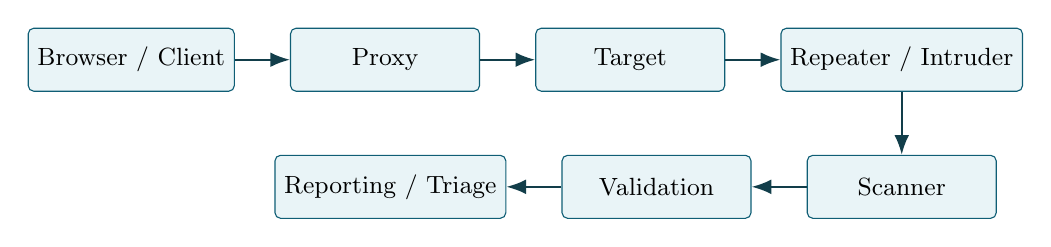
\begin{tikzpicture}[
  node distance=8mm and 7mm,
  every node/.style={font=\small},
  box/.style={draw=accent, rounded corners=2pt, fill=accentlight, minimum width=2.4cm, minimum height=0.8cm, align=center},
  arrow/.style={-{Latex[length=2.5mm]}, thick, draw=accentdark}
]
  \node[box] (browser) {Browser / Client};
  \node[box, right=of browser] (proxy) {Proxy};
  \node[box, right=of proxy] (target) {Target};
  \node[box, right=of target] (manual) {Repeater / Intruder};
  \node[box, below=of manual] (scanner) {Scanner};
  \node[box, left=of scanner] (validate) {Validation};
  \node[box, left=of validate] (report) {Reporting / Triage};

  \draw[arrow] (browser) -- (proxy);
  \draw[arrow] (proxy) -- (target);
  \draw[arrow] (target) -- (manual);
  \draw[arrow] (manual) -- (scanner);
  \draw[arrow] (scanner) -- (validate);
  \draw[arrow] (validate) -- (report);
\end{tikzpicture}
\end{center}

\subsection{Proxy}

Proxy captures HTTP, HTTPS, and WebSocket traffic passing between the client and the application. Requests and responses can be inspected, modified, forwarded, dropped, or routed to other Burp tools.

\subsection{Target}

Target maintains information about the application's attack surface, including scope, the site map, discovered resources, and crawl paths. It provides the structural context used to organize testing activity.

\subsection{Repeater}

Repeater provides an interactive environment for modifying and resending individual HTTP or WebSocket messages. Common AppSec uses include:

\begin{itemize}
  \item Authentication and session testing.
  \item Authorization and IDOR/BOLA testing.
  \item Parameter tampering and boundary testing.
  \item Business-logic investigation.
  \item Vulnerability validation and reproduction.
\end{itemize}

\subsection{Intruder}

Intruder automates customized request generation and payload injection. Typical uses include fuzzing parameters, enumerating identifiers, testing input validation, and exercising request permutations during authorized assessments.

\subsection{Scanner}

Burp Scanner is PortSwigger's DAST engine. Its principal activities are \textbf{crawling} and \textbf{auditing}. Crawling discovers reachable functionality and navigation paths; auditing analyzes requests and application behavior for vulnerabilities.

% -----------------------------------------------------------------------------
\section{Burp Collaborator and OAST}

\subsection{Why Out-of-Band Testing Matters}

Some vulnerabilities produce no useful evidence in the HTTP response that triggered them. The application may instead perform asynchronous processing or cause a backend system to communicate with an external service.

Burp Collaborator supports \textbf{Out-of-Band Application Security Testing (OAST)} by issuing unique interaction identifiers and observing whether the target produces external DNS, HTTP, or other supported callbacks.

\begin{center}
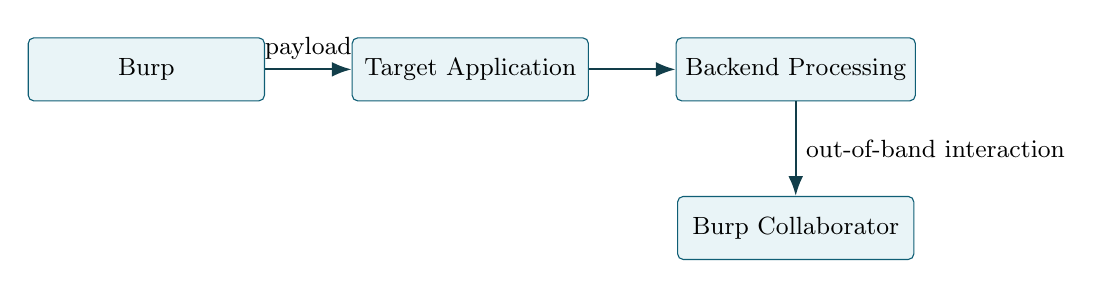
\begin{tikzpicture}[
  node distance=12mm and 11mm,
  every node/.style={font=\small},
  box/.style={draw=accent, rounded corners=2pt, fill=accentlight, minimum width=3.0cm, minimum height=0.8cm, align=center},
  arrow/.style={-{Latex[length=2.5mm]}, thick, draw=accentdark}
]
  \node[box] (burp) {Burp};
  \node[box, right=of burp] (app) {Target Application};
  \node[box, right=of app] (backend) {Backend Processing};
  \node[box, below=of backend] (collab) {Burp Collaborator};

  \draw[arrow] (burp) -- node[above]{payload} (app);
  \draw[arrow] (app) -- (backend);
  \draw[arrow] (backend) -- node[right]{out-of-band interaction} (collab);
\end{tikzpicture}
\end{center}

\subsection{Common OAST Use Cases}

Collaborator is especially useful for testing classes of vulnerabilities where direct responses may be absent or misleading, including:

\begin{itemize}
  \item Blind SSRF.
  \item Blind XXE.
  \item Blind command injection.
  \item Blind XSS.
  \item Server-side template or expression injection with outbound interaction.
  \item Asynchronous backend processing flaws.
  \item External URL-fetching weaknesses.
\end{itemize}

\subsection{Automated and Manual Use}

Burp Scanner can use Collaborator automatically for multiple scan checks. Burp Suite Professional also provides a Collaborator client for manually generating payloads, inserting them into candidate injection points, polling for interactions, and analyzing the resulting evidence.

\subsection{Private Collaborator Infrastructure}

Organizations with sensitive data-handling requirements can deploy private Collaborator infrastructure. This is useful for internal applications, restricted networks, regulated environments, or cases where external interaction data must remain within enterprise-controlled infrastructure.

% -----------------------------------------------------------------------------
\section{Extensions and the Montoya API}

\subsection{Extension Architecture}

Burp extensions customize Burp beyond its built-in functionality. Extensions can inspect or modify traffic, generate requests, add user-interface elements, integrate external systems, enrich findings, or automate repetitive testing tasks.

\subsection{Montoya API}

The \textbf{Montoya API} is PortSwigger's modern extension API. Java is the primary supported implementation language, with Kotlin also suitable when compiled into compatible JAR packages. The older Extender API remains relevant for legacy extension ecosystems but should not be the default choice for new engineering work.

\begin{center}
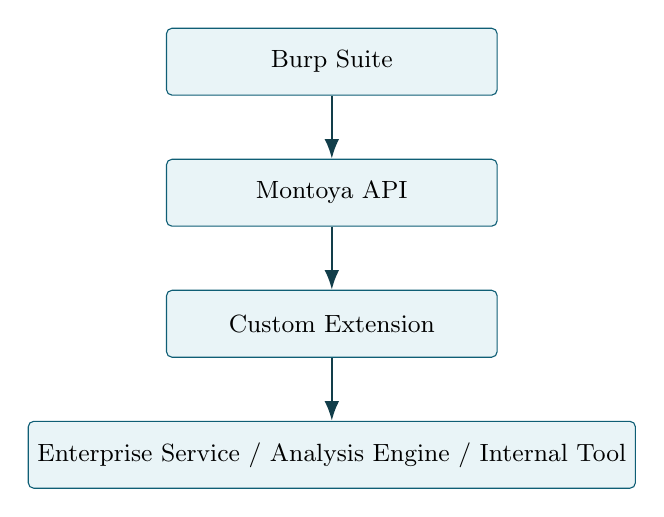
\begin{tikzpicture}[
  node distance=8mm,
  every node/.style={font=\small},
  box/.style={draw=accent, rounded corners=2pt, fill=accentlight, minimum width=4.2cm, minimum height=0.85cm, align=center},
  arrow/.style={-{Latex[length=2.5mm]}, thick, draw=accentdark}
]
  \node[box] (burp) {Burp Suite};
  \node[box, below=of burp] (api) {Montoya API};
  \node[box, below=of api] (ext) {Custom Extension};
  \node[box, below=of ext] (enterprise) {Enterprise Service / Analysis Engine / Internal Tool};

  \draw[arrow] (burp) -- (api);
  \draw[arrow] (api) -- (ext);
  \draw[arrow] (ext) -- (enterprise);
\end{tikzpicture}
\end{center}

\subsection{Practical AppSec Engineering Uses}

Examples include:

\begin{itemize}
  \item \textbf{Ticketing integration:} convert validated findings into vulnerability-management records.
  \item \textbf{Finding enrichment:} add asset criticality, ownership, or internal risk metadata.
  \item \textbf{Authorization testing:} transform identity context and compare responses across roles.
  \item \textbf{Policy enforcement:} detect organization-specific header, cookie, or response requirements.
  \item \textbf{Security telemetry:} export testing events to enterprise logging or analytics systems.
\end{itemize}

\subsection{AI-Enabled Extensions}

Montoya-based extensions can use Burp's managed AI capabilities. Security engineers should treat model output as untrusted and design extension workflows defensively against prompt injection, malformed output, and over-privileged automation.

% -----------------------------------------------------------------------------
\section{API Security Scanning}

Modern applications often expose large portions of their security-sensitive functionality through APIs. Burp Scanner supports direct API discovery and auditing from supported definitions and live endpoints.

\subsection{Supported Definition Types}

\begin{table}[htbp]
\centering
\caption{API definition and discovery support}
\begin{tabularx}{\textwidth}{@{}lX@{}}
\toprule
\textbf{Technology / Format} & \textbf{Support Model} \\
\midrule
OpenAPI 3.x & Definition-driven API scanning using JSON or YAML specifications. \\
Swagger 2.0 & Supported for legacy OpenAPI-style API definitions. \\
Postman Collection 2.1 & Collection-driven endpoint and request discovery. \\
SOAP / WSDL & Service discovery and test generation from WSDL definitions. \\
GraphQL & Live schema discovery using introspection when enabled by the target. \\
\bottomrule
\end{tabularx}
\end{table}

\subsection{API-Only Scan Flow}

\begin{center}
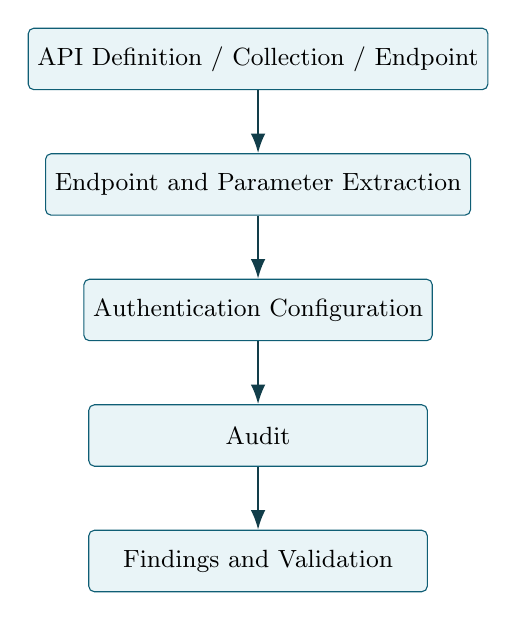
\begin{tikzpicture}[
  node distance=8mm,
  every node/.style={font=\small},
  box/.style={draw=accent, rounded corners=2pt, fill=accentlight, minimum width=4.3cm, minimum height=0.78cm, align=center},
  arrow/.style={-{Latex[length=2.5mm]}, thick, draw=accentdark}
]
  \node[box] (def) {API Definition / Collection / Endpoint};
  \node[box, below=of def] (extract) {Endpoint and Parameter Extraction};
  \node[box, below=of extract] (auth) {Authentication Configuration};
  \node[box, below=of auth] (audit) {Audit};
  \node[box, below=of audit] (findings) {Findings and Validation};

  \draw[arrow] (def) -- (extract);
  \draw[arrow] (extract) -- (auth);
  \draw[arrow] (auth) -- (audit);
  \draw[arrow] (audit) -- (findings);
\end{tikzpicture}
\end{center}

\subsection{API Authentication}

Common mechanisms include HTTP Basic authentication, bearer tokens, and API keys. The correct credential model should be associated with the API's declared or operational authentication mechanism before auditing.

\subsection{Automation Limits}

Automated API scanning should be supplemented with manual testing for issues that depend on application semantics and identity context, including:

\begin{itemize}
  \item Broken Object Level Authorization (BOLA).
  \item Broken Function Level Authorization (BFLA).
  \item Excessive data exposure.
  \item Mass assignment.
  \item Improper property-level authorization.
  \item Multi-step authorization weaknesses.
  \item Tenant-isolation failures.
  \item Business-logic vulnerabilities.
\end{itemize}

\begin{practicebox}[Engineering practice]
Use schema-driven scanning to maximize deterministic endpoint coverage, then use role-aware manual testing to investigate authorization and business-logic conditions that cannot be inferred from the API contract alone.
\end{practicebox}

% -----------------------------------------------------------------------------
\section{Authenticated Scanning}

\subsection{Why Authenticated Coverage Matters}

Anonymous scanning may expose only a fraction of an application's attack surface. Authenticated scanning is needed to reach account dashboards, administrative interfaces, internal workflows, user-specific APIs, and other protected functions.

\subsection{Authentication Methods}

Burp supports direct credential-based authentication as well as recorded login sequences for more complex workflows.

Recorded login sequences are particularly useful for:

\begin{itemize}
  \item Single Sign-On (SSO).
  \item Multi-step authentication.
  \item Additional login fields.
  \item TOTP-based MFA.
  \item WebAuthn-related flows.
\end{itemize}

\subsection{Role Coverage}

For applications with multiple authorization tiers, consider separate scans or validation passes for distinct identities:

\begin{center}
\begin{tabular}{@{}llll@{}}
\toprule
Anonymous & Standard User & Privileged User & Administrator \\
\bottomrule
\end{tabular}
\end{center}

Comparing reachable functions and server behavior across identities helps expose authorization gaps that a single authenticated scan may miss.

% -----------------------------------------------------------------------------
\section{Session Handling and Application State}

Authentication establishes identity; session handling maintains that identity and any required application state across later requests.

\subsection{Session Handling Rules}

Burp's Sessions configuration supports session handling rules composed of:

\begin{center}
\textbf{Scope + Actions}
\end{center}

The scope determines where the rule applies. Actions control how outgoing requests are prepared.

Common actions include:

\begin{itemize}
  \item Adding cookies from Burp's cookie jar.
  \item Setting cookies, parameters, or headers.
  \item Validating whether the current session remains authenticated.
  \item Running a macro.
  \item Running post-request macros.
  \item Invoking an extension.
  \item Performing browser-assisted session recovery.
\end{itemize}

\subsection{Macros}

A macro is a predefined sequence of requests that Burp can execute to establish or refresh application state.

\begin{lstlisting}[style=guidecode]
GET /login
  -> extract anti-CSRF token
POST /login
  -> submit username, password, anti-CSRF token
HTTP 302 /dashboard
  -> capture authenticated session cookie
Subsequent request
  -> inject refreshed state
\end{lstlisting}

Macros are useful when an application dynamically generates CSRF tokens, session identifiers, workflow tokens, or other request-dependent state.

\subsection{Cookie Jar}

Burp's cookie jar tracks cookies discovered through supported tools and can update later requests during interactive testing workflows.

\subsection{Scanner-Specific Distinction}

\begin{warningbox}[Important distinction]
Burp Scanner manages session state during crawl-driven scanning differently from the traditional desktop session-handling workflow. For automated Scanner authentication, recorded login sequences and scan authentication configuration are generally the appropriate mechanisms.
\end{warningbox}

% -----------------------------------------------------------------------------
\section{Passive, Active, and JavaScript Security Analysis}

Burp Scanner uses several distinct analysis strategies.

\subsection{Passive Analysis}

Passive checks inspect observed traffic without generating attack requests. Typical findings include insecure headers, cookie weaknesses, information disclosure, and sensitive data exposed in responses.

\subsection{Active Analysis}

Active checks deliberately modify requests and observe the application's behavior. Their operational impact varies by check type and configuration.

\begin{table}[htbp]
\centering
\caption{Practical scan-intensity model}
\begin{tabularx}{\textwidth}{@{}lXl@{}}
\toprule
\textbf{Mode} & \textbf{Operational Characteristic} & \textbf{Relative Risk} \\
\midrule
Passive & Analyze existing traffic only. & Low \\
Light Active & Limited additional requests with relatively low expected impact. & Low--Moderate \\
Medium Active & More aggressive input mutation and attack-style behavior. & Moderate \\
Intrusive & Tests that may alter state, data, or availability. & High \\
\bottomrule
\end{tabularx}
\end{table}

\subsection{JavaScript Analysis}

Burp can use static and dynamic analysis techniques for client-side code and DOM-based vulnerability detection.

\subsection{Live Tasks}

Two useful live task concepts are:

\begin{itemize}
  \item \textbf{Live audit:} performs vulnerability auditing on selected or observed requests.
  \item \textbf{Live passive crawl:} adds observed resources and structure to the Target site map.
\end{itemize}

\begin{warningbox}[Do not conflate these concepts]
A live passive crawl is primarily an attack-surface discovery activity. It should not be interpreted as equivalent to passive vulnerability scanning.
\end{warningbox}

% -----------------------------------------------------------------------------
\section{BChecks and Custom Vulnerability Detection}

\subsection{Purpose}

\textbf{BChecks} allow AppSec teams to define custom Scanner checks without building a complete Java extension. Each check is stored as a plain-text \texttt{.bcheck} file using PortSwigger's BCheck definition language.

BChecks can encode organization-specific security knowledge such as:

\begin{itemize}
  \item Deprecated endpoint detection.
  \item Internal secret formats.
  \item Forbidden framework versions.
  \item Required security headers.
  \item Debug interfaces.
  \item Internal metadata leakage.
  \item Product-specific vulnerability patterns.
  \item Newly disclosed vulnerabilities awaiting native Scanner coverage.
\end{itemize}

\subsection{Conceptual Passive Check}

\begin{center}
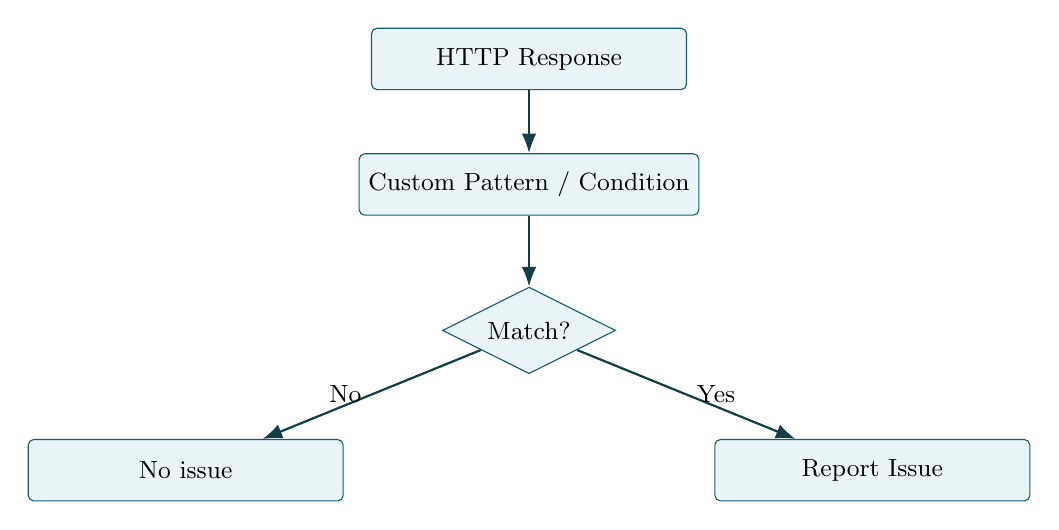
\begin{tikzpicture}[
  node distance=8mm,
  every node/.style={font=\small},
  box/.style={draw=accent, rounded corners=2pt, fill=accentlight, minimum width=4.0cm, minimum height=0.78cm, align=center},
  decisionnode/.style={diamond, draw=accent, fill=accentlight, aspect=2, align=center},
  arrow/.style={-{Latex[length=2.5mm]}, thick, draw=accentdark}
]
  \node[box] (resp) {HTTP Response};
  \node[box, below=of resp] (pattern) {Custom Pattern / Condition};
  \node[decisionnode, below=of pattern, yshift=-1mm] (match) {Match?};
  \node[box, below left=11mm and 18mm of match] (no) {No issue};
  \node[box, below right=11mm and 18mm of match] (yes) {Report Issue};

  \draw[arrow] (resp) -- (pattern);
  \draw[arrow] (pattern) -- (match);
  \draw[arrow] (match) -- node[left]{No} (no);
  \draw[arrow] (match) -- node[right]{Yes} (yes);
\end{tikzpicture}
\end{center}

\begin{keypointbox}[Institutional knowledge as code]
BChecks provide a lightweight mechanism for turning recurring security research and organization-specific detection requirements into repeatable automated checks.
\end{keypointbox}

% -----------------------------------------------------------------------------
\section{CI/CD Integration and DevSecOps}

Burp Suite DAST provides the primary Burp architecture for enterprise-scale CI/CD integration.

\subsection{CI-Driven Scan Pattern}

\begin{center}
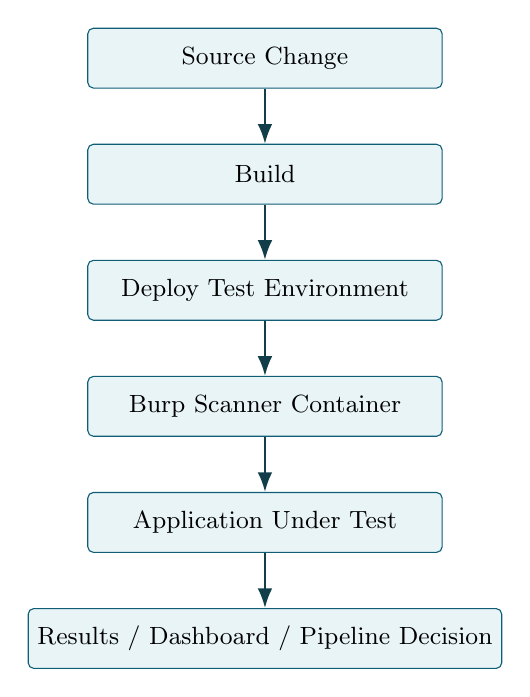
\begin{tikzpicture}[
  node distance=7mm,
  every node/.style={font=\small},
  box/.style={draw=accent, rounded corners=2pt, fill=accentlight, minimum width=4.5cm, minimum height=0.76cm, align=center},
  arrow/.style={-{Latex[length=2.5mm]}, thick, draw=accentdark}
]
  \node[box] (change) {Source Change};
  \node[box, below=of change] (build) {Build};
  \node[box, below=of build] (deploy) {Deploy Test Environment};
  \node[box, below=of deploy] (scanner) {Burp Scanner Container};
  \node[box, below=of scanner] (app) {Application Under Test};
  \node[box, below=of app] (results) {Results / Dashboard / Pipeline Decision};

  \draw[arrow] (change) -- (build);
  \draw[arrow] (build) -- (deploy);
  \draw[arrow] (deploy) -- (scanner);
  \draw[arrow] (scanner) -- (app);
  \draw[arrow] (app) -- (results);
\end{tikzpicture}
\end{center}

\subsection{Integration Targets}

Container-driven scanning can be integrated into CI systems that can run Docker workloads. Typical enterprise targets include GitHub Actions, Jenkins, TeamCity, Azure DevOps, CircleCI, and Bamboo.

\subsection{Configuration as Code}

CI-driven scanning can use YAML-based configuration for elements such as:

\begin{itemize}
  \item Start URLs.
  \item Scope.
  \item Scan configuration.
  \item Authentication details.
  \item Custom BChecks and extensions.
\end{itemize}

\subsection{Recommended Pipeline Strategy}

A mature AppSec pipeline distinguishes between fast feedback and deep assessment.

\begin{table}[htbp]
\centering
\caption{Layered DAST execution model}
\begin{tabularx}{\textwidth}{@{}lX@{}}
\toprule
\textbf{Pipeline Stage} & \textbf{Suggested Security Activity} \\
\midrule
Pull request & Fast targeted security checks and high-confidence regression coverage. \\
Integration environment & CI-optimized DAST with bounded runtime and risk. \\
Nightly / scheduled & Broader authenticated crawling and auditing. \\
Pre-production & Deeper active scanning under controlled conditions. \\
Manual assessment & Business logic, authorization, exploit validation, and edge-case testing. \\
\bottomrule
\end{tabularx}
\end{table}

\begin{practicebox}[Build-breaking policy]
Do not treat every DAST result identically. A robust policy considers severity, confidence, exploitability, duplicate state, accepted risk, application criticality, and whether a finding has been manually validated.
\end{practicebox}

% -----------------------------------------------------------------------------
\section{Burp AI}

Burp AI provides AI assistance inside selected Burp workflows while the security engineer retains primary control of the testing process.

Capabilities may include:

\begin{itemize}
  \item Contextual assistance in Repeater.
  \item Explanation of unfamiliar headers, cookies, JavaScript, and protocol constructs.
  \item Additional investigation of Scanner findings.
  \item Assistance with recorded login creation.
  \item AI-powered custom actions.
  \item AI capabilities exposed to supported extensions through the Montoya API.
\end{itemize}

\begin{warningbox}[Security handling]
AI-generated output should be treated as untrusted. Security engineers should validate model conclusions, constrain privileges, review generated requests before high-impact actions, and account for prompt-injection risks when application-controlled content is included in AI context.
\end{warningbox}

% -----------------------------------------------------------------------------
\section{Burp AT: Agentic Application Security Testing}

\subsection{Agentic Model}

Burp AT extends Burp from task-level assistance toward agentic testing. Instead of receiving only a single transformation or analysis request, the agent can work toward a higher-level security objective by selecting and orchestrating multiple Burp capabilities.

A representative workflow is:

\begin{center}
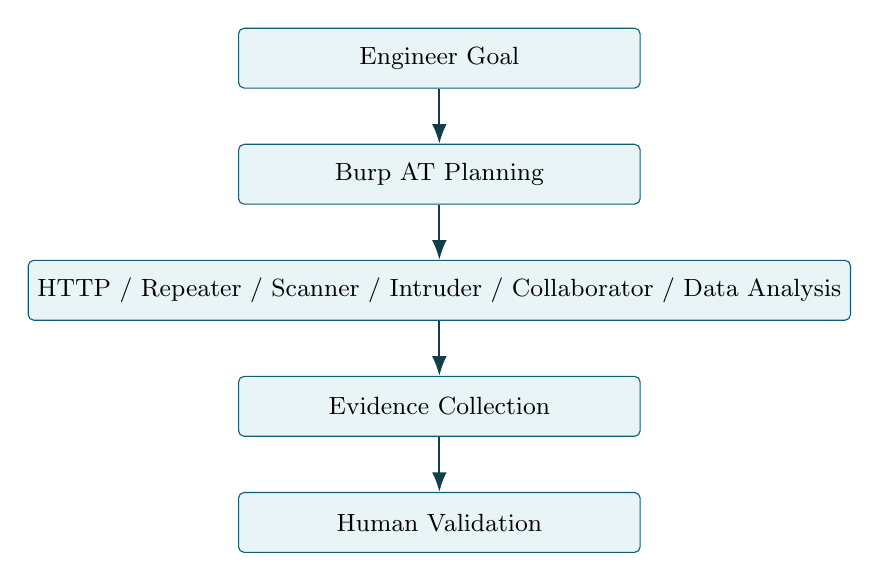
\begin{tikzpicture}[
  node distance=7mm,
  every node/.style={font=\small},
  box/.style={draw=accent, rounded corners=2pt, fill=accentlight, minimum width=5.1cm, minimum height=0.76cm, align=center},
  arrow/.style={-{Latex[length=2.5mm]}, thick, draw=accentdark}
]
  \node[box] (goal) {Engineer Goal};
  \node[box, below=of goal] (plan) {Burp AT Planning};
  \node[box, below=of plan] (tools) {HTTP / Repeater / Scanner / Intruder / Collaborator / Data Analysis};
  \node[box, below=of tools] (evidence) {Evidence Collection};
  \node[box, below=of evidence] (review) {Human Validation};

  \draw[arrow] (goal) -- (plan);
  \draw[arrow] (plan) -- (tools);
  \draw[arrow] (tools) -- (evidence);
  \draw[arrow] (evidence) -- (review);
\end{tikzpicture}
\end{center}

\subsection{Tool Categories}

Burp AT can orchestrate capabilities spanning areas such as:

\begin{itemize}
  \item Scanning and auditing.
  \item Scope and site-map analysis.
  \item HTTP requests and responses.
  \item Vulnerability issue review.
  \item Custom scan checks.
  \item Datasets and scripting.
  \item Intruder-based fuzzing.
  \item Burp Collaborator.
  \item Encoding and decoding operations.
\end{itemize}

\subsection{Autonomy Controls}

Agentic workflows should be governed by explicit permissions and scope. A secure operating model allows routine actions to execute automatically while preserving approval boundaries for higher-impact activity.

\subsection{Human Validation Remains Mandatory}

Agentic automation does not replace application context, threat modeling, or engineering judgment. The security engineer remains responsible for validating:

\begin{itemize}
  \item Whether observed behavior represents a real vulnerability.
  \item Whether exploitation assumptions are technically valid.
  \item Whether authorization boundaries were modeled correctly.
  \item Whether the testing method respected production-safety constraints.
  \item Whether the impact statement reflects the application's actual business context.
  \item Whether the proposed remediation addresses root cause rather than symptoms.
\end{itemize}

% -----------------------------------------------------------------------------
\section{Integrated AppSec Operating Model}

The capabilities described in this guide fit naturally into a layered security engineering workflow.

\begin{center}
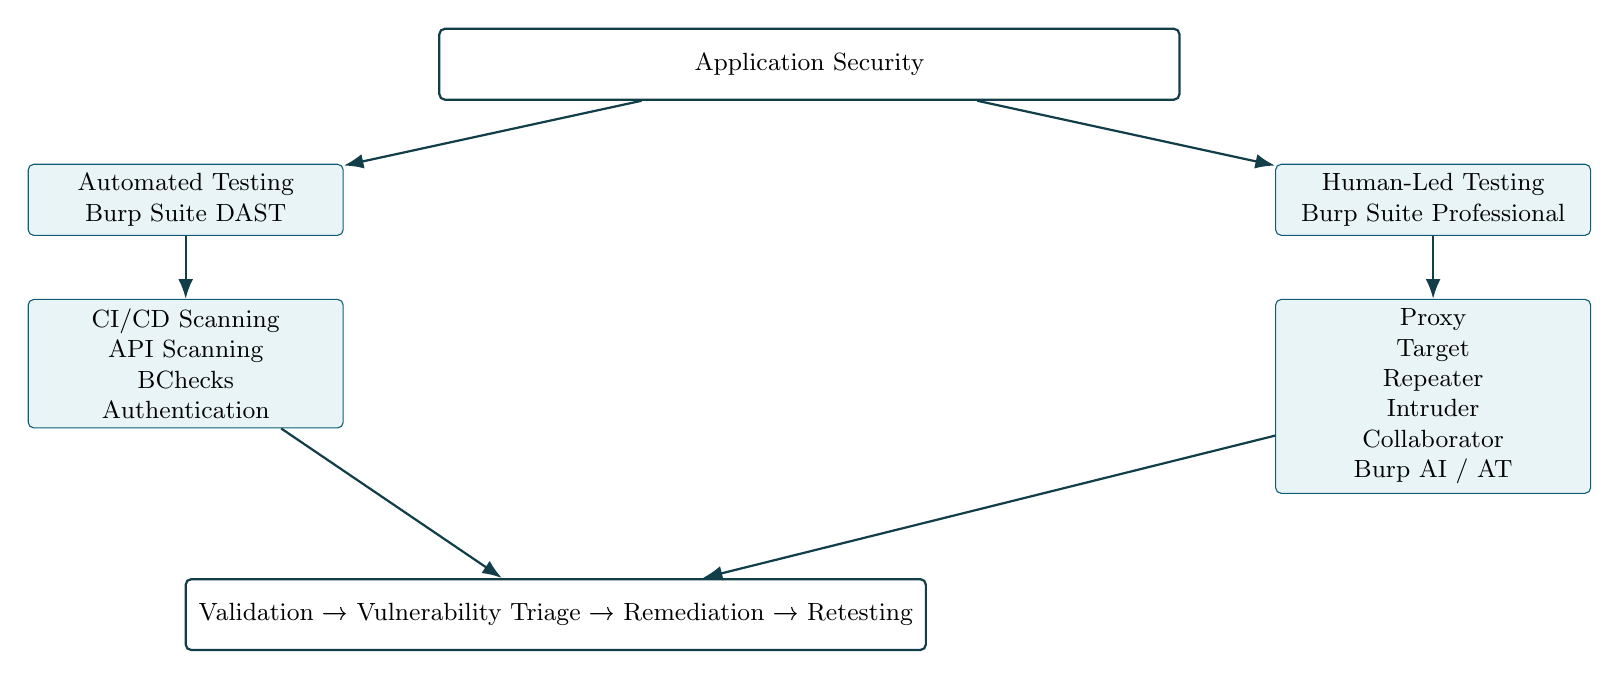
\begin{tikzpicture}[
  node distance=8mm and 12mm,
  every node/.style={font=\small},
  box/.style={draw=accent, rounded corners=2pt, fill=accentlight, minimum width=4.0cm, minimum height=0.8cm, align=center},
  bigbox/.style={draw=accentdark, rounded corners=2pt, fill=white, minimum width=9.4cm, minimum height=0.9cm, align=center, thick},
  arrow/.style={-{Latex[length=2.5mm]}, thick, draw=accentdark}
]
  \node[bigbox] (appsec) {Application Security};
  \node[box, below left=of appsec] (auto) {Automated Testing\\Burp Suite DAST};
  \node[box, below right=of appsec] (human) {Human-Led Testing\\Burp Suite Professional};
  \node[box, below=of auto] (auto2) {CI/CD Scanning\\API Scanning\\BChecks\\Authentication};
  \node[box, below=of human] (human2) {Proxy\\Target\\Repeater\\Intruder\\Collaborator\\Burp AI / AT};
  \node[bigbox, below=19mm of auto2, xshift=47mm] (validation) {Validation \textrightarrow{} Vulnerability Triage \textrightarrow{} Remediation \textrightarrow{} Retesting};

  \draw[arrow] (appsec) -- (auto);
  \draw[arrow] (appsec) -- (human);
  \draw[arrow] (auto) -- (auto2);
  \draw[arrow] (human) -- (human2);
  \draw[arrow] (auto2) -- (validation);
  \draw[arrow] (human2) -- (validation);
\end{tikzpicture}
\end{center}

\subsection{Operational Sequence}

A useful mental model is:

\begin{enumerate}
  \item \textbf{Intercept} --- understand the application's real traffic.
  \item \textbf{Map} --- identify the reachable attack surface.
  \item \textbf{Authenticate} --- expose protected functionality.
  \item \textbf{Audit} --- combine passive, active, and JavaScript analysis.
  \item \textbf{Extend} --- add organization-specific detection with BChecks and Montoya.
  \item \textbf{Detect out-of-band behavior} --- use Collaborator/OAST.
  \item \textbf{Validate} --- reproduce findings through manual testing.
  \item \textbf{Automate} --- integrate Burp Suite DAST with CI/CD.
  \item \textbf{Augment} --- use Burp AI for focused assistance.
  \item \textbf{Orchestrate} --- use Burp AT for controlled multi-step agentic testing.
\end{enumerate}

\begin{keypointbox}[Final engineering principle]
The objective is not to maximize the number of tools used. The objective is to combine deterministic automation, manual analysis, application context, and repeatable engineering controls so that findings are accurate, reproducible, and actionable.
\end{keypointbox}

% -----------------------------------------------------------------------------
\section{Official Documentation References}

The following PortSwigger documentation pages are recommended as primary references for implementation details and product behavior. Product features evolve, so operational guidance should be checked against the current documentation before production deployment.

\begin{enumerate}
  \item Burp Scanner: \url{https://portswigger.net/burp/documentation/scanner}
  \item Burp Collaborator: \url{https://portswigger.net/burp/documentation/collaborator}
  \item Collaborator client: \url{https://portswigger.net/burp/documentation/desktop/tools/collaborator}
  \item Burp extensions: \url{https://portswigger.net/burp/documentation/desktop/extend-burp/extensions}
  \item Creating extensions / Montoya API: \url{https://portswigger.net/burp/documentation/desktop/extend-burp/extensions/creating}
  \item AI-enabled extensions: \url{https://portswigger.net/burp/documentation/desktop/extend-burp/extensions/creating/creating-ai-extensions}
  \item API scanning: \url{https://portswigger.net/burp/documentation/desktop/running-scans/api-scans}
  \item API scanning FAQ: \url{https://portswigger.net/burp/documentation/scanner/api-scanning-faq}
  \item Authenticated scanning: \url{https://portswigger.net/burp/documentation/scanner/authenticated-scanning}
  \item Recorded login sequences: \url{https://portswigger.net/burp/documentation/scanner/authenticated-scanning/recorded-login-sequences}
  \item Sessions settings: \url{https://portswigger.net/burp/documentation/desktop/settings/sessions}
  \item Macros: \url{https://portswigger.net/burp/documentation/desktop/settings/sessions/macros}
  \item Scanner auditing: \url{https://portswigger.net/burp/documentation/scanner/auditing}
  \item Audit settings: \url{https://portswigger.net/burp/documentation/scanner/scan-configurations/audit-settings}
  \item Live tasks: \url{https://portswigger.net/burp/documentation/desktop/running-scans/live-tasks}
  \item BChecks: \url{https://portswigger.net/burp/documentation/scanner/bchecks}
  \item BCheck worked examples: \url{https://portswigger.net/burp/documentation/scanner/bchecks/worked-examples}
  \item CI-driven scans: \url{https://portswigger.net/burp/documentation/dast/user-guide/ci-cd/ci-driven-scans}
  \item Built-in Scanner configurations: \url{https://portswigger.net/burp/documentation/scanner/scan-configurations/burp-scanner-built-in-configs}
  \item Burp AI: \url{https://portswigger.net/burp/documentation/desktop/burp-ai}
  \item Burp AT: \url{https://portswigger.net/burp/documentation/desktop/burp-at}
  \item Burp AT tools: \url{https://portswigger.net/burp/documentation/desktop/burp-at/tools}
  \item Burp AT permissions: \url{https://portswigger.net/burp/documentation/desktop/burp-at/permissions}
\end{enumerate}

\vfill
\begin{center}
  \small\color{muted}
  Use Burp Suite only against systems for which you have explicit authorization to test.
\end{center}

\end{document}
